% 
% (c) 2015, Florian Mayer
%
% This document is released under the terms
% of the GNU Free Documentation License
%
% See LICENSE for further information regarding
% this license.
%%

\documentclass[11pt,a4paper]{article}
\usepackage{listings,palatino,avant,graphicx,color,pslatex}
\usepackage[ngerman]{babel}
\usepackage[margin=2cm]{geometry}
\usepackage{courier}
\usepackage[table]{xcolor}
\usepackage[utf8]{inputenc}
\usepackage{graphicx}
\usepackage{lmodern}
\usepackage{amsmath}
\usepackage{bytefield}
\usepackage[colorlinks=true,linkcolor=black,citecolor=black,urlcolor=black]{hyperref}

\definecolor{lightblue}{rgb}{0.2925,0.6381,0.65}
\definecolor{darkblue}{rgb}{0.0105,0.2764,0.35}
\definecolor{grey}{gray}{0.75}

\lstset{numbers=none,numberstyle=\small\ttfamily,stepnumber=1,numbersep=4pt}
\lstset{tabsize=4}
\lstset{breaklines=true, breakatwhitespace=true}
\lstset{frame=none}

\lstdefinestyle{c}
	{language=C, identifierstyle=\color{darkblue},
	 basicstyle=\small\ttfamily, keywordstyle=\color{lightblue}\bfseries,
	 commentstyle=\color{grey}}

\lstdefinestyle{bash}
	{basicstyle=\small\ttfamily,language=bash, 
	 identifierstyle=\color{darkblue}}

\def\inlinebash{\lstinline[style=bash]}
\def\inlinec{\lstinline[style=c]}

\begin{document}
\title{\color{black} Ext4-Übung}
\author{\color{darkblue} Florian Mayer}
\maketitle

\tableofcontents

\section{Einführung}
Im ersten Kapitel dieses Dokuments werden die 
Werkzeuge des e2fsprogs-Pakets näher beleuchtet.
Danach folgt die eigentliche Übung

\subsection{Bestandteile des e2fsprogs-Pakets}
Die Tools -- soweit nicht anders vermerkt -- arbeiten 
jeweils mit ext2, ext3 oder ext4 Dateisystemen. ``ExtX'' bezeichnet
zusammenfassend ext2- ext3- oder ext4-Systeme.

\paragraph{e2fsk}
	Überprüft ein ExtX-System auf Inkonsistenzen und behebt diese, wenn möglich.

\paragraph{mke2fs}
	Wird vom Frontendprogramm \inlinebash$mkfs$ verwendet um neue ExtX-Dateisysteme anzulegen.

\paragraph{resize2fs}
	Kann genutzt werden, um ein ExtX-Dateisystem an eine gewachsene oder
	verkleinerte Partition anzupassen.

\paragraph{tune2fs}
	Setzt oder modifiziert Dateisystemparameter.

\paragraph{dumpe2fs}
	Schreibt Superblock- bzw. Blockgruppeninformationen auf die Standardausgabe.

\paragraph{filefrag}
	Zeigt den Grad der Dateifragmentierung an.

\paragraph{e2label}
	Verändert das Dateisystemlabel eines ExtX-Systems.

\paragraph{findfs}
	Sucht nach einem Dateisystem mit einem Label oder einer UUID.

\paragraph{e2freefrag}
	Wie \inlinebash$filefrag$, jedoch mit dem Unterschied, dass nur die Fragmentierung
	des freien Speicherplatzes aufgezeigt wird.

\paragraph{chattr}
	Ähnlich zu \inlinebash$chmod$ oder \inlinebash$chown$. Funktioniert auf vielen verschiedenen Dateisystemen. 

\paragraph{e2image}
	Speichert kritische ExtX-Metadaten in einer Datei. 

\paragraph{e4defrag}
	Defragmentiert ein Ext4-Dateisystem während es parallel
	weiterhin genutzt werden kann.

\paragraph{findsuper}
	Findet Ext2-Superblocks. Veraltet und lt. Dokumentation ``schnell zusammengehackt''.

\subsection{Verwendete Programme}
Im Rahmen dieses Dokuments werden lediglich die Programme \inlinebash$debugfs$
und \inlinebash$dumpe2fs$ verwendet. Die Manualseiten könnten, wie gewohnt, mit
\begin{lstlisting}[style=bash]
$ man debugfs
$ man dumpe2fs
\end{lstlisting}
angesehen werden. Das Studium dieser Handbücher ist dringend empfohlen.

\section{Übung}

\subsection{Vorbereitungen des Test-Dateisystems}

Operationen auf Dateisysteme mit sog. Debugging-Kommandos
sind gefährlich. Löscht man z.B. versehentlich einen Inode, so
ist es nur noch schwer möglich die zugehörige Datei wiederherzustellen. 
Es wird daher beschrieben, wie eine sog.
Sandbox-Umgebung (also ein vom System abgekapseltes Dateisystem)
eingerichtet werden kann. Die hier geschilderte Methode steht
sofort unter GNU/Linux zur Verfügung, da sie integraler Kernel-Bestandteil ist.

\begin{itemize}
\item \inlinebash$dd if=/dev/zero of=~/foo.disk count=1000$\\
	Erzeugt eine genullte Datei, bestehend aus 1000 Blöcken zu jeweils 0,5KiB.

\item \inlinebash$losetup --list$\\
	Zeigt bereits vorhandene loop devices (footnote) an. Bereits vorhandene Loop-Geräte
	müssen mittels \inlinebash$sudo losetup -d /dev/loop<X>$ ausgehängt werden. 

\item \inlinebash$sudo losetup /dev/loop0 ~/foo.disk$\\
	Erzeugt eine blockorientierte Gerätedatei, die alle Lese- und Schreiboperationen
	auf die Datei \~/foo.disk abbildet. Das Kommando muss sodann mithilfe von
	\inlinebash$losetup --list$ überprüft werden. Der Vorgang war erfolgreich, 
	wenn nun die neue Konfiguration ausgegeben wird.

\item \inlinebash$sudo parted /dev/loop0 mklabel msdos$\\
	Erstellt eine Partitionstabelle mit \emph{msdos}-Format. Das bedeutet, dass
	ein normaler MBR erstellt wird.
	
\item \inlinebash$sudo parted /dev/loop0 mkpart primary 0 500K$\\
	Das erste Kommando erzeugt einen neuen MBR und das zweite
	richtet eine primäre Partition über die volle Länge des
	virtuellen Blockgeräts ein.

\item \inlinebash$sudo mkfs.ext4 /dev/loop0p1$\\
	Erzeugt das zu untersuchende Dateisystem. Achtung: Hier darf
	/dev/loop0 nicht verwendet werden, da dies keine Partition ist!
	Die Gerätedatei der Partition (\emph{/dev/loop0p1}) wird automatisch
	vom System erkannt und steht daher sofort nach Erzeugung der
	Partition zur Verfügung.

\item
Nun muss das frische Dateisystem nur noch eingebunden werden:

\begin{lstlisting}[style=bash]
$ sudo su
$ mkdir /mnt/foo
$ mount /dev/loop0p1 /mnt/foo
\end{lstlisting}
\end{itemize}

\subsection{Allgemeine Fragen}
\begin{enumerate}
\item Wo liegt der Superblock, bzw. ab welchem Offset beginnt dieser.
	Wie groß ist er? Hinweis: Der Superblock enthält eine sog. Magic-Number
	die 2 Bytes groß ist und ab Offset 0x38 beginnt.
\item Wieviel Inodes und Datenblöcke wurden beim Erstellen des Dateisystems erzeugt?
	Hinweis: Die Ausgabe des \inlinebash$mkfs.ext4$ Kommandos hilft. Alternativ 
	kann auch \inlinebash$dumpe2fs$ benutzt werden.
\item Wie groß ist ein Ext4-Datenblock und wie viele sind davon anfangs
	tatsächlich durch Dateien nutzbar? Hinweis: Nutzen Sie \inlinebash$dumpe2fs$
\item Wieviele Bytes ist ein Inode groß? Hinweis: Nutzen Sie wieder \inlinebash$dumpe2fs$

\end{enumerate}

\subsection{Dumpe2fs}
	Beantworten Sie mithilfe des Programms \inlinebash$dumpe2fs$ 
	die folgenden Fragen unter der Annahme,
	dass Sie sich auf einem \emph{32-Bit-System} 
	befinden\footnote{Tatsächlich werden Sie jedoch auf 
		einem 64-Bit-System arbeiten}.
	\begin{enumerate}
		\item Über wie viele Bytes erstreckt sich ein ext4-Block?
			Hinweis: Sie müssen nach ``Block size:'' suchen.
		\item Wie groß kann das Dateisystem maximal werden? 
			Hinweis: Multiplizieren Sie die Blockgröße 
			mit der maximalen Anzahl der Blöcke. Beachten Sie die Wortgröße!
		\item Wie viele Inodes kann es maximal geben? Hinweis: 
			Jeder Inode hat eine 4-Byte-Inode-Nummer und keine zwei Inodes
			dürfen dieselbe ID tragen.
		\item Wie groß kann eine Datei, die in eine einzige Block-Gruppe passt,
			maximal sein? Hinweis: Die Ausgabe von \inlinebash$dumpe2fs$ liefert
			einen Eintrag, der auf die Menge der Datenblöcke innerhalb einer
			Blockgruppe Aufschluss gibt.
	\end{enumerate}

\subsection{Einlesen des Superblocks}
Schreiben Sie ein C-Programm mit dem sie den Superblock einlesen und
einige Informationen auf der Kommandozeile ausgeben.

\begin{itemize}
	\item Anzahl der Inodes
	\item Insgesamte Anzahl der Blöcke
	\item Erster Datenblock
	\item Anzahl freier Inodes
	\item Anzahl freier Datenblöcke
	\item Magic Number (Ausgabe in Hex)
	\item 128-bit UUID des Dateisystems (Ausgabe in Hex)
	\item Betriebssystem des Erstellers
\end{itemize}

\begin{lstlisting}[style=c]
/* Blaupause fuer die Loesung */
#include <ext2fs/ext2fs.h>
#include <ext2fs/ext2_fs.h>
#include <stdio.h>
#include <stdlib.h>
#include <et/com_err.h>
#include <stdint.h>

static const char DEV[] = "/dev/loop0p1";
static const char OS_L[] = "LINUX";
static const char OS_O[] = "OTHER";

int main(int argc, char **argv){
	errcode_t err;
	ext2_filsys fs;
	struct ext2_super_block *super;

	/* Oeffnen des Dateisystemhandles "fs" mithilfe der Funktion ext2fs_open.
		Signatur der Funktion ist: errcode_t ext2fs_open(const char *name,
			int flags, int superblock, int block_size, io_manager manager,
			ext2_filsys *filsys);
		Fuer "flags" koennen Sie EXT2_FLAG_RW, fuer "superblock" und "block_size" 0
		und fuer "io_manager" koennen Sie unix_io_manager einsetzen. */
	??? 

	if (err){
		if (err == 13) {
			printf("[ext2fs_open] Insufficient permissions\n");
		} else {
			printf("[ext2fs_open] Error number: %ld\n", err);
		}
		return EXIT_FAILURE;
	}
	
	super = fs->super;	

	/* Hier printf-Statements der folgenden Member von super:
		super->s_inodes_count super->s_blocks_count
		super->s_first_data_block super->s_free_inodes_count
		super->s_free_blocks_count super->s_magic
		super->s_uuid[] super->s_creator_os */
	???

	/* Schliessen des Dateisystem-Handles mittels ext2fs_close(fs) */
	???

	if (err){
		printf("[ext2fs_close] Error number: %ld\n", err);
		return EXIT_FAILURE;
	}

	return EXIT_SUCCESS;
}
\end{lstlisting}

\subsection{Anlegen von Testdaten}

\begin{enumerate}
\item Erstellen Sie im neuen Dateisystem den angegebenen Verzeichnisbaum 
	mithilfe der Werkzeuge \inlinebash$touch$, \inlinebash$mkdir$ und 
	\inlinebash$nano$\slash\inlinebash$echo$. Hierfür steht ihnen ein Bash-Skript 
	zur Verfügung. Der Aufruf ist unten in der Baumansicht aufgeführt.

\begin{verbatim}
/+-> t1
 |   +-> dirA
 |      +-> foo.txt  -- Inhalt: "FOO.TXT"
 |   +-> a.txt -- Inhalt "A"
 |   +-> b.txt -- Inhalt "B" 
 |   +-> c.txt 
 +-> t2
 |   +-> dirB
 |   +-> dirC
 +-> foo.txt -- Inhalt "FOO"
 
\end{verbatim}
\end{enumerate}

\subsection{Debugfs}
In dieser Aufgabe machen Sie sich mit dem Dateisystemdebugger
\inlinebash$debugfs$ vertraut.

\begin{enumerate}
	\item Starten Sie debugfs (\inlinebash$debugfs /dev/loop0p1$).
	\item Welcher Inode stellt das Verzeichnis ``t1'' dar, welcher ``t2''?
		(Hinweis \inlinebash$ls -l$\footnote{
			Es handelt sich hierbei um ein Kommando von \emph{debugfs}, ist also
			insbesondere nicht mit dem \emph{ls}-Kommando zu verwechseln.})
	\item Welcher Inode stellt die Verzeichniswurzel dar und
		auf welchem Block (i.S.v. Ext4) liegt dieser?
		(Hinweis \inlinebash$imap <inode nummer> ODER <pfad>$)
	\item Wechseln Sie mit \inlinebash$cd$ in das Verzeichnis ``t1'' und lassen
		Sie sich alle Inodes anzeigen. Benutzen Sie das ``cat''-
		Kommando, um sich den Inhalt der Dateien a.txt und b.txt
		ausgeben zu lassen.
	\item Wo liegt der Block des Inodes für a.txt?
	\item Lassen Sie sich mittels \inlinebash$stat <inode nummer>$ den
		Inodestatus für die Datei a.txt ausgeben.
		Auf welchem Block liegen die Daten?
	\item Geben Sie den Datenblock mittels \inlinebash$block_dump$ aus.
	\item Wie viele Blocks benötigt die Datei c.txt?
		(Hinweis: \inlinebash$blocks <inode nummer>$)
	\item Geben sie auch noch einen der ausgegebenen Blöcke
		auf der Standardausgabe aus (\inlinebash$block_dump$).
\end{enumerate}

\subsection{Inodes}
\begin{enumerate}
	\item Lassen Sie sich Inode der Datei \emph{a.txt} mithilfe der Kommandos \inlinebash$dd$
		und \inlinebash$hexdump$ anzeigen. Hinweis: Suchen Sie zunächst die Nummer des Inodes.
		Nun können Sie die Blocknummer des Inodes und dessen Offset zu diesem Block ermitteln.
		Erinnern Sie sich auch daran, dass ein Inode typischerweise 128 Byte groß sein wird!
	\item Schreiben Sie ein C-Programm mit dem Sie sich die folgenden Daten
		des Inodes der Datei \emph{c.txt} ausgeben lassen.
		\begin{itemize}
			\item User-ID
			\item Erstellungsdatum (nicht formatiert, am besten in hex ausgeben)
			\item Zugriffsdatum (ebenfalls nicht formatiert)
			\item Berechtigungen (Dateimodus)
			\item Anzahl der Hardlinks
			\item Dateigröße in Bytes
		\end{itemize}
		
	\item Schreiben Sie ein zweites Programm mit dessen Hilfe sie die 
		Berechtigungen des eben ausgelesenen Inodes auf den Modus 777, 
		und die UID auf 4711 setzen.
		Eine Sinnhaftigkeit dieser Veränderung sei dahingestellt.
\end{enumerate}

\section{Blockgruppen Layout von Ext4}
Die folgende Tabelle beschreibt den grundsätzlichen Aufbau einer ext4-Blockgruppe.
Die Menge der Blöcke, die in einer Blockgruppe enthalten sind, lässt sich leicht
mithilfe des \inlinebash$dumpe2fs$-Kommandos ermitteln (vgl. auch 2.3).
\paragraph{}

\begin{table}[h]
	\begin{center}
		\begin{tabular}[c]{| l | l |}
			\hline
			\cellcolor{grey} Daten & \cellcolor{grey} Größe \\ \hline
			Füllbytes vor der Gruppe 0 & 1024 Bytes \\ \hline
			Super Block & 1 Block (1KiB, 2KiB, 4KiB, \ldots, 64KiB) \\ \hline
			Group-Descriptors & n Blöcke  \\ \hline
			Reservierte Group-Descriptors & k Blöcke. Werden für's nachträgliche Vergrößern benötigt \\ \hline
			Datenblock Bitmap & 1 Block \\ \hline
			Inode Bitmap & 1 Block \\ \hline
			Inode Tabelle & j Blöcke (Im Test-Dateisystem 8 1KiB-Blöcke) \\ \hline
			Datenblöcke & Der Rest \\ \hline
		
		\end{tabular}
	\end{center}

	\caption{Blockgruppen Layouttabelle}
	\label{tab:block_layout}
\end{table}

\begin{figure}[h]
	\centering
	\caption{Blockgruppenlayout}
	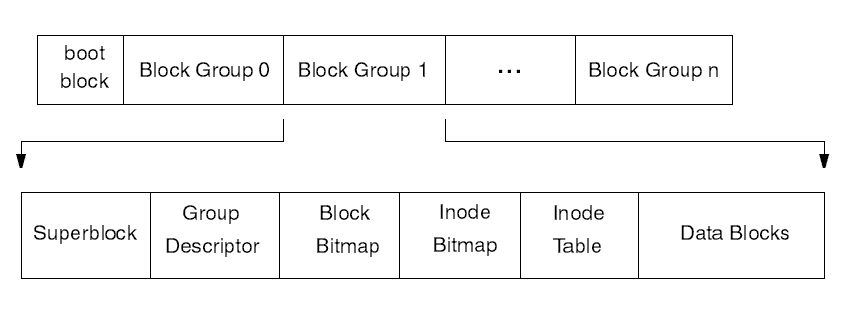
\includegraphics[scale=0.4]{images/block_group_layout.png}
	\label{fig:block_group}
\end{figure}

\end{document}
